\subsection{Laufzeitvergleiche}
\hypertarget{Sec:Laufzeit}{}

In diesem Kapitel wollen wir die Dauer der Berechnung der Momente mit verschiedenen Methoden vergleichen. Für alle Berechnung wurden möglichst gleiche Voraussetzungen geschaffen, indem möglichst alle Programme im Hintergrund geschlossen wurden.

\begin{Beispiel}{(Laufzeit Exponentialverteilung)}
Sei $X \sim \Exp(\lambda)$ mit $\lambda > 0$ exponentialverteilt. Der folgende Graph stellt die Dauer für die Berechnung der ersten hundert Momente dar.

\begin{figure}[H]
\centering
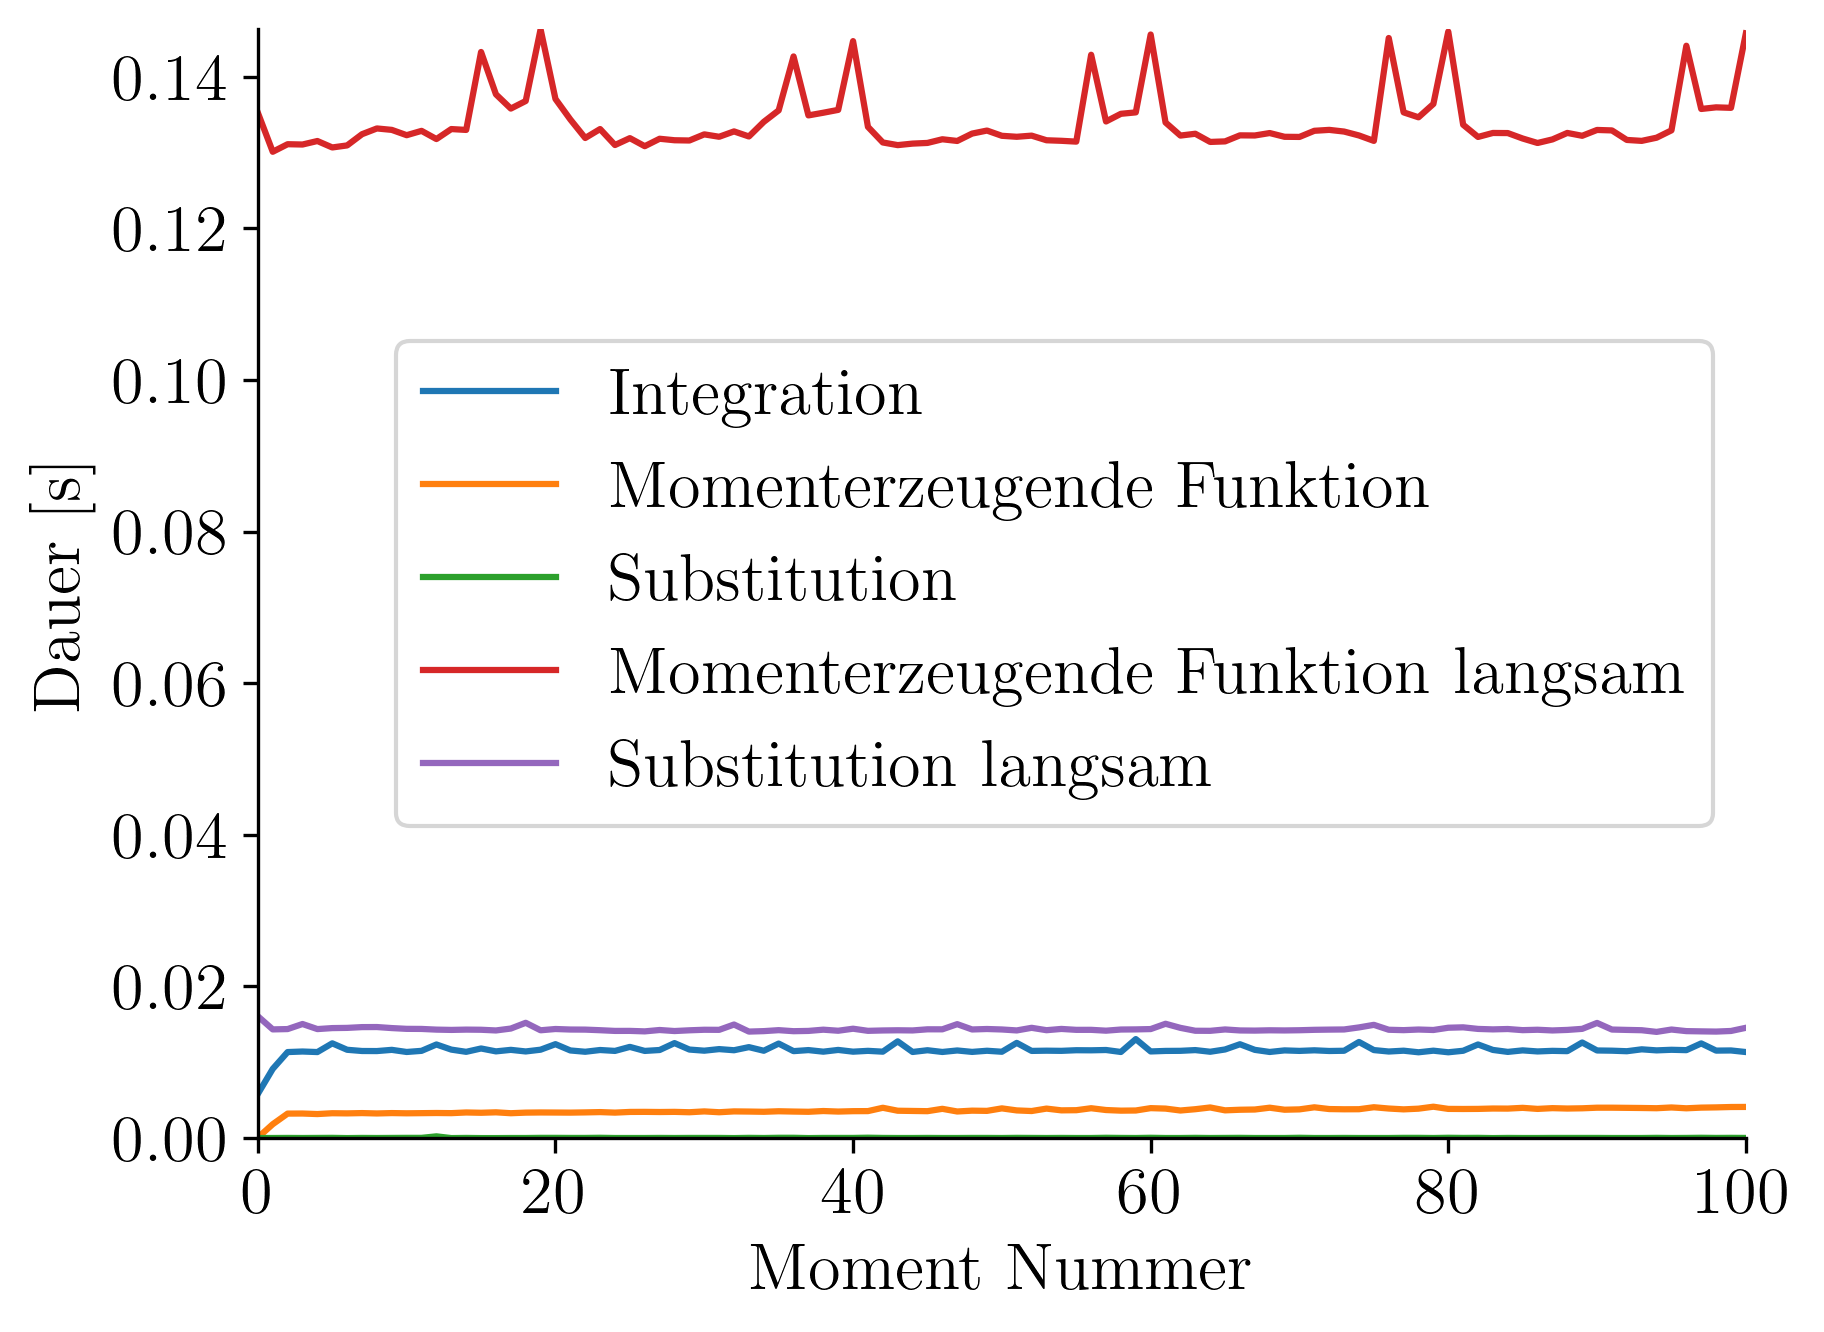
\includegraphics[width=0.5\linewidth]{./Section/Momente/Dauer Exp.png}
\vspace*{-.3\baselineskip}
\caption{Dauer der Berechnung der ersten hundert Momente einer $\Exp(\lambda)$-Verteilung}
\end{figure}

Für die Erstellung der Daten lassen wir die ersten hundert Momente hundertmal berechnen. Für Integration verwenden wir die \lstinline|_moment_integration|- und für momenterzeugende Funktion die \lstinline|_moment_generating|-Methode. Für die langsam-Kurven wird vor jeder Berechnung das \lstinline|MGF|-Attribut gelöscht. Somit muss dort jedes Mal die momenterzeugende Funktion neu berechnet werden. Für Substitution wird zu Beginn (ohne Messung der Zeit) das $n$-te Momente berechnet und anschließend für $n$ der entsprechende Wert eingesetzt. Im langsamen Fall wird das $n$-te Moment für jede Iteration von neuem berechnet.\\

Interessant sind die Spitzen bei $[15, 19]$, $[36, 40]$, $[56, 60]$ sowie $[76, 80]$ und $[96, 100]$. Dies dauert circa $10 \%$ länger, als die anderen Berechnungen. Es kann nicht am Ableiten liegen, da sonst die ähnliche Doppelspitzen auch in der Kurve für die optimierte Berechnung mit der momenterzeugenden Funktion zu finden wären. Der Garbage Collector kann mit ziemlicher Sicherheit ausgeschlossen werden, da nach jeder Berechnung der Inhalt der Variable mit \lstinline|del| gelöscht wird. Verwenden wir einen anderen Computer, so erhalten wir

\begin{figure}[H]
\centering
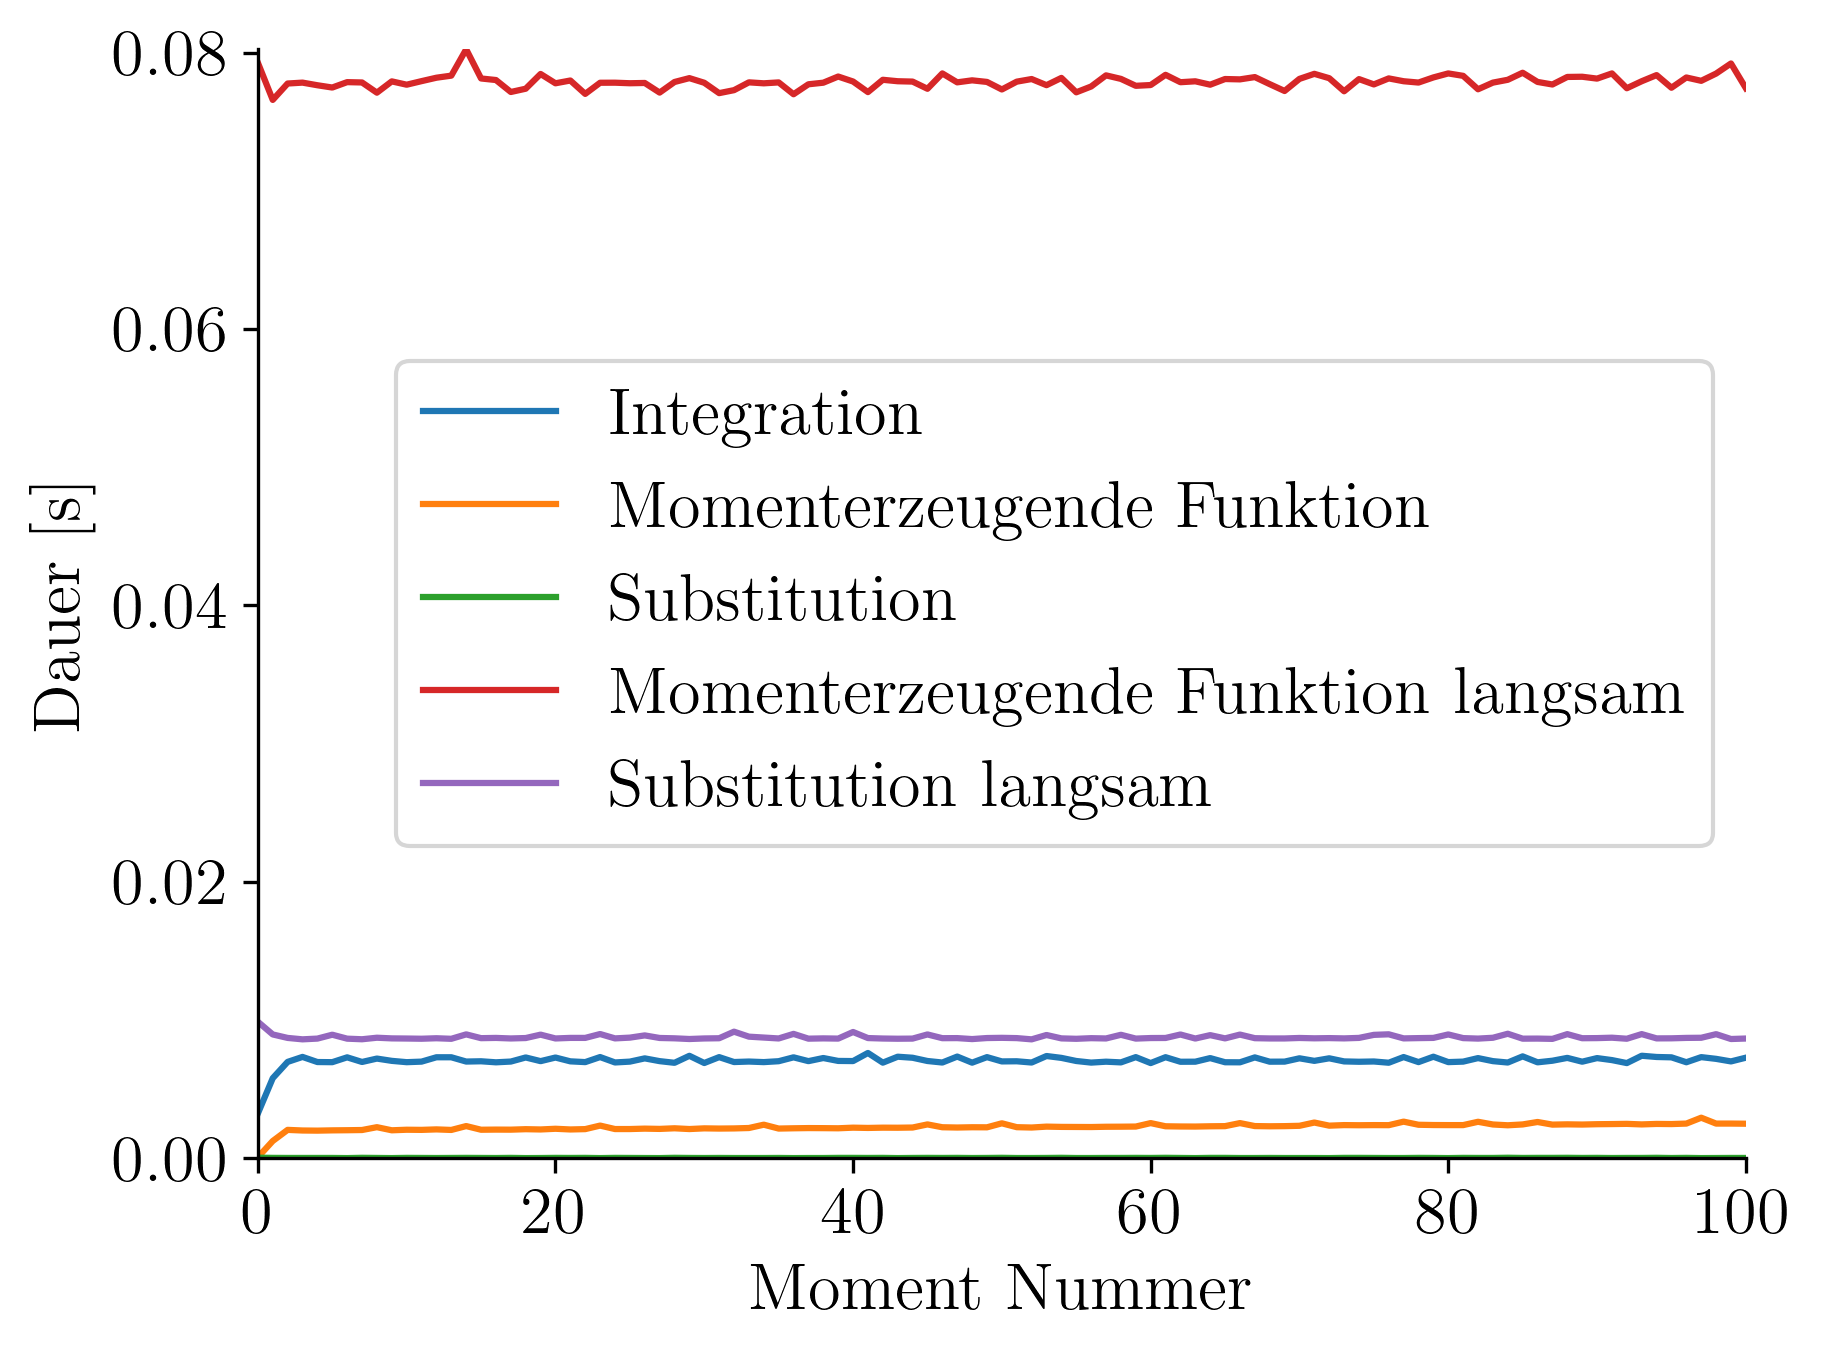
\includegraphics[width=0.5\linewidth]{./Section/Momente/Dauer Exp Alex.png}
\vspace*{-.3\baselineskip}
\caption{Dauer der Berechnung der ersten hundert Momente einer $\Exp(\lambda)$-Verteilung}
\end{figure}

An dieser Grafik lässt sich feststellen, dass das erste System um etwa die Hälfte langsamer ist als das zweite. Zudem treten die angesprochenen Spitzen nicht erneut auf. Daraus lässt sich schließen, dass diese Anomalie vermutlich nichts mit dem Programm selbst zu tun hat.\\

Für die folgende Diskussion werden wir uns mit den ersten Daten beschäftigen. Um den Graphen zu vereinfachen, ist die folgende Grafik linear interpoliert.

\begin{figure}[H]
\centering
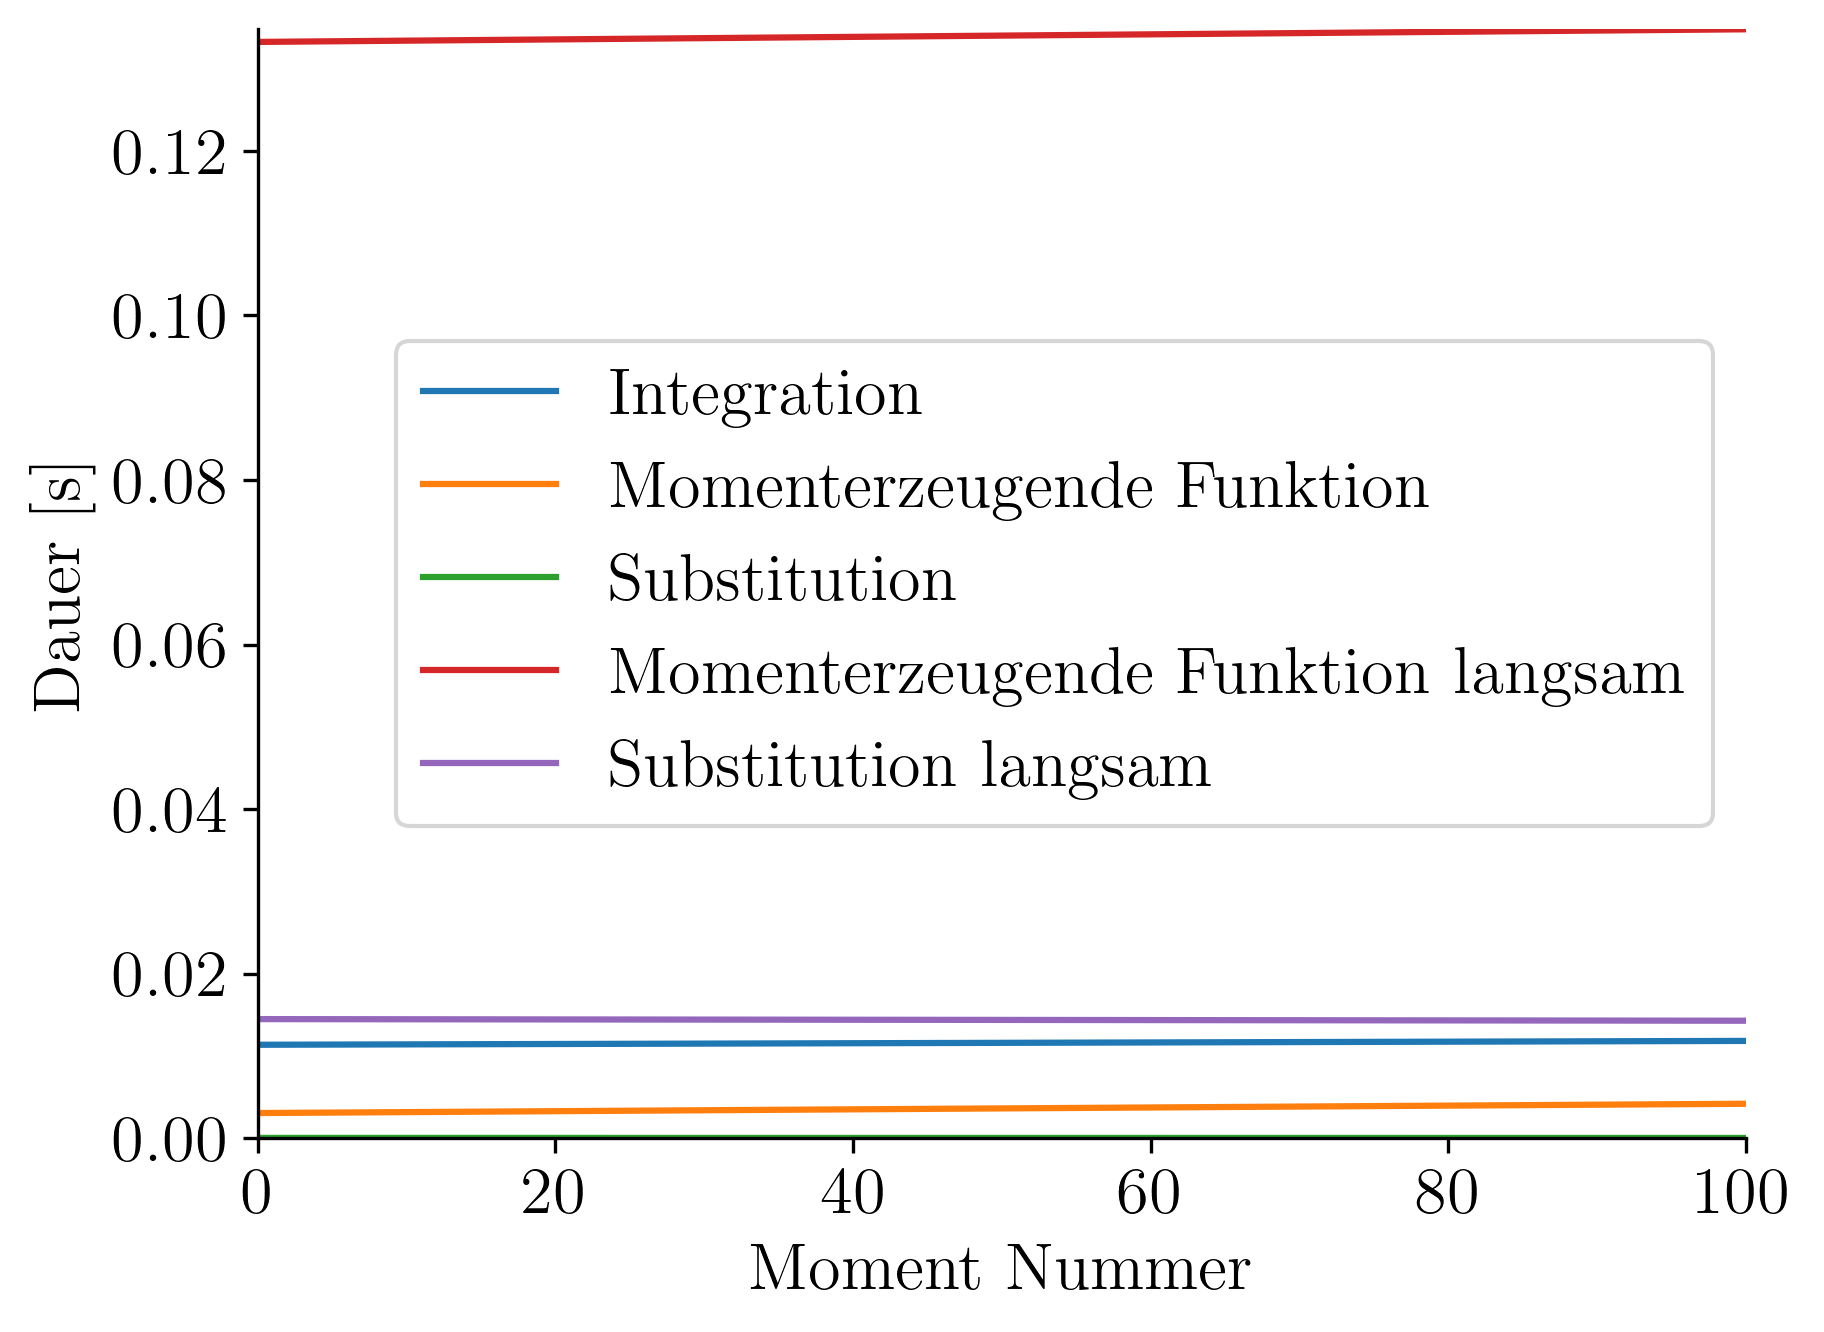
\includegraphics[width=0.5\linewidth]{./Section/Momente/Dauer Exp Lin.png}
\vspace*{-.3\baselineskip}
\caption{Interpolierte Dauer der Berechnung der ersten hundert Momente einer $\Exp(\lambda)$-Verteilung}
\end{figure}

Betrachten wir den Unterschied zwischen den beiden Geraden für die momenterzeugende Funktion, so erhalten wir eine Dauer von $0.1310$ Sekunden. Lassen wir die momenterzeugende Funktion eintausendmal berechnen, so erhalten wir im Mittel einen Wert von $0.1362$ Sekunden. Dies stimmt also mit obigem Abstand überein. Da die Berechnung der momenterzeugende Funktion scheinbar eine \glqq teure\grqq{} Berechnung ist, ist es sinnvoll die momenterzeugende Funktion, falls sie schon berechnet wurde, in dem Attribut \lstinline|MGF| zu speichern. Dies findet analog für die kumulantenerzeugende Funktion unter \lstinline|CGF| und die im folgenden Kapitel vorgestellt charakteristische Funktion unter \lstinline|CF| statt.\\

Für diese Zufallsvariable macht es scheinbar keinen großen Unterschied, mit welcher Methode man die Momente berechnet. Es ist allerdings sehr interessant, dass die Berechnung der Momente mittels Substitution, falls zuvor das $n$-te Moment berechnet quasi instantan stattfindet. Man könnte sich an dieser Stelle wundern, wieso es keine Methode gibt, die ein Moment mittels Substitution berechnet. Die Berechnung des $n$-ten Moments ist für die meisten Verteilungen höchst aufwendig und für viele Verteilungen kann SymPy auch keinen geschlossenen Ausdruck angeben. Des Weiteren haben wir, wie bei dem \hyperlink{Bsp:Nicht-Int}{\blue{Beispiel zur nicht-integrierbaren Familie}} gesehen, auch ein Problem, falls das $n$-te Moment eine stückweise Funktion ist. Es fällt auf, dass die Berechnung mithilfe der momenterzeugenden Funktion um circa $0.008$ Sekunden schneller ist, als die Berechnung mittels Integration. Daher scheint es momentan eher unsinnvoll zu sein die Integration als Standardmethode gewählt zu haben. Weiter fällt auf, dass alle Methoden nahezu konstanten Aufwand haben. Die Steigung ist jeweils im Bereich von $10^{-6}$, was vermutlich auf Messungenauigkeiten zurückzuführen ist.
\end{Beispiel}

\vspace*{-\medskipamount}

\newpage

\begin{Beispiel}{(Laufzeit Normalverteilung)}
Sei $X \sim \Nor(\mu, \sigma)$ mit $\mu, \sigma > 0$ normalverteilt. Da die Berechnungen hier deutlich mehr Zeit in Anspruch nehmen, lassen wir die ersten hundert Momente nur zehnmal berechnen und  verzichten auf die unoptimierten Varianten der Berechnungen.

\begin{figure}[H]
\centering
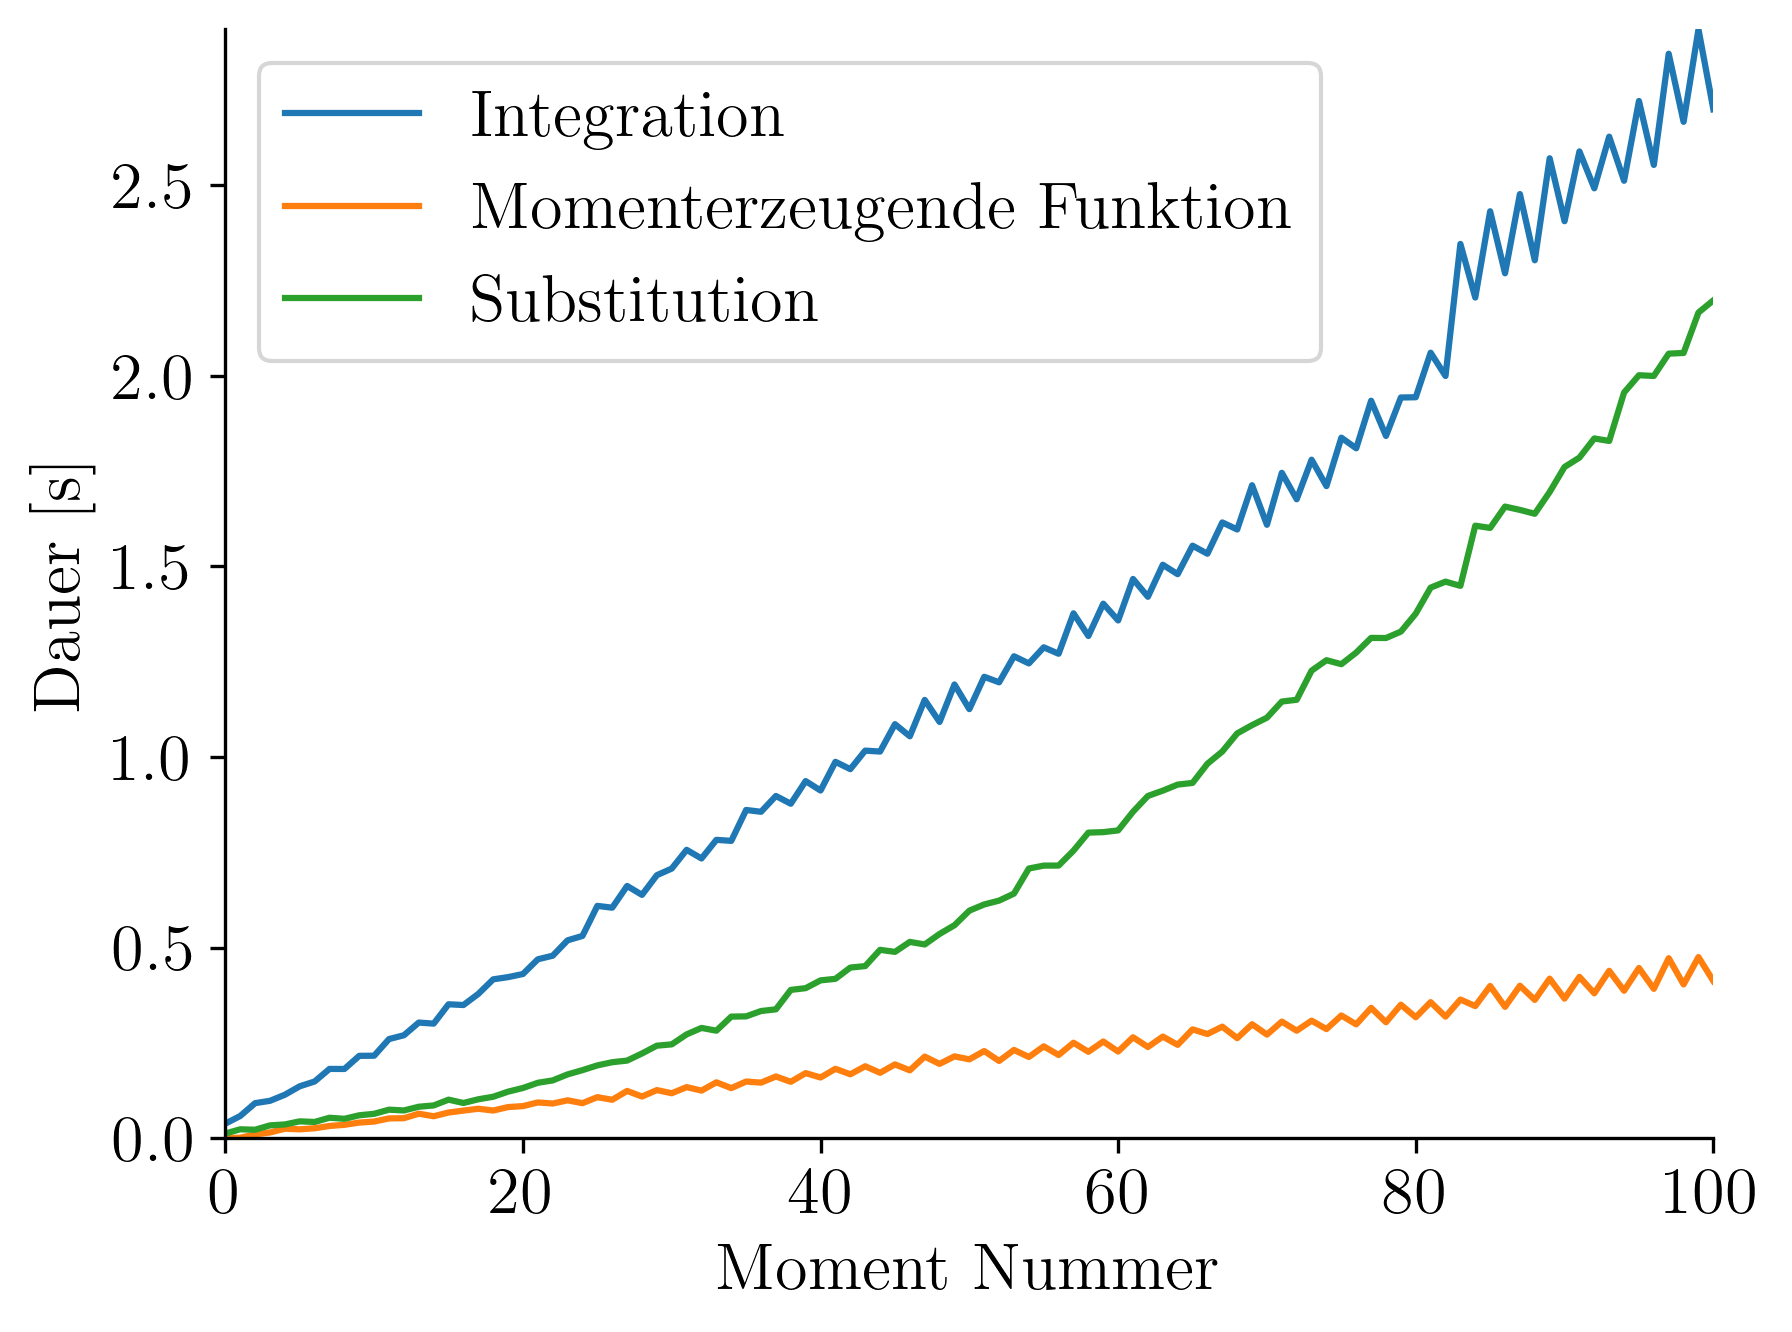
\includegraphics[width=0.5\linewidth]{./Section/Momente/Dauer Nor Falsch.png}
\vspace*{-.3\baselineskip}
\caption{Dauer der Berechnung der ersten hundert Momente einer $\Nor(\mu, \sigma)$-Verteilung ohne Vereinfachung}
\end{figure}

Dieser Plot spiegelt aber nicht ganz die Wahrheit wieder. Lassen wir mit SymPy das $n$-te Moment berechnen, so erhalten wir
\[\mathbb{E}(X^n) = \frac{2^{\frac{n}{2} - 1} \sigma^{n} \left(\left(-1\right)^{n} {G_{1, 2}^{2, 1}\left(\begin{matrix} \frac{1}{2} - \frac{n}{2} &  \\0, \frac{1}{2} &  \end{matrix} \middle| {\frac{\mu^{2}}{2 \sigma^{2}}} \right)} + {G_{1, 2}^{2, 1}\left(\begin{matrix} \frac{1}{2} - \frac{n}{2} &  \\0, \frac{1}{2} &  \end{matrix} \middle| {\frac{\mu^{2} e^{2 i \pi}}{2 \sigma^{2}}} \right)}\right) e^{- \frac{\mu^{2}}{2 \sigma^{2}}}}{\pi}~.\]
Setzen wir beispielsweise den Wert $n = 6$ ein, so erhalten wir
\[\mathbb{E}(X^6) = \frac{2 \sigma^{4} \left({G_{1, 2}^{2, 1}\left(\begin{matrix} - \frac{3}{2} &  \\0, \frac{1}{2} &  \end{matrix} \middle| {\frac{\mu^{2}}{2 \sigma^{2}}} \right)} + {G_{1, 2}^{2, 1}\left(\begin{matrix} - \frac{3}{2} &  \\0, \frac{1}{2} &  \end{matrix} \middle| {\frac{\mu^{2} e^{2 i \pi}}{2 \sigma^{2}}} \right)}\right) e^{- \frac{\mu^{2}}{2 \sigma^{2}}}}{\pi}~.\]
Wir wollen eigentlich den Ausdruck
\[\mathbb{E}(X^6) = \mu^6 + 15 \mu^4 \sigma^2 + 45 \mu^2 \sigma^4 + 15 \sigma^6~.\]
Diesen erhalten wir durch die Anwendung von \lstinline|simplify| auf obigen Ausdruck. Verwenden wir diesen Schritt auch in der obigen Berechnung, so erhalten wir das folgende Bild.

\begin{figure}[H]
\centering
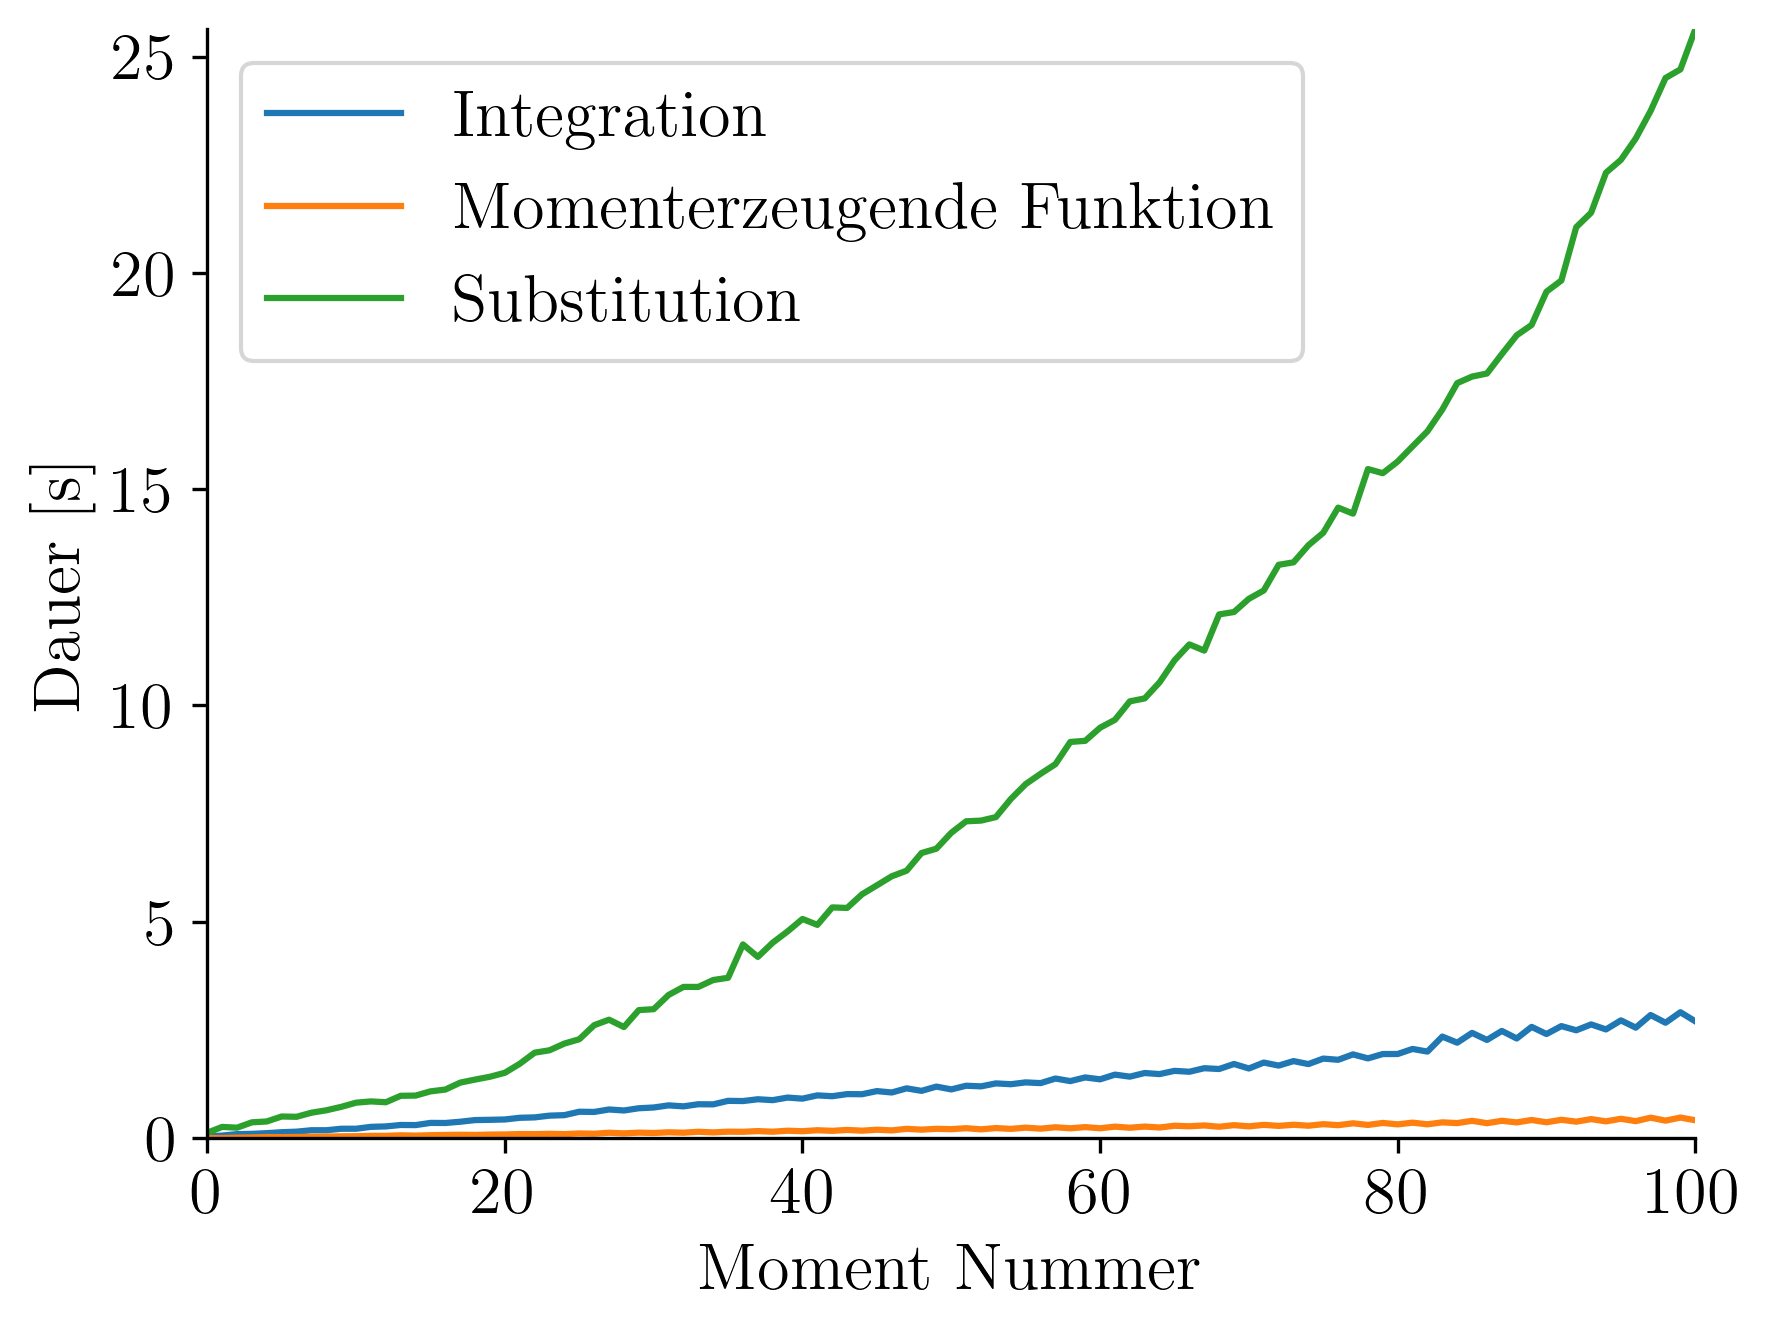
\includegraphics[width=0.5\linewidth]{./Section/Momente/Dauer Nor.png}
\vspace*{-.3\baselineskip}
\caption{Dauer der Berechnung der ersten hundert Momente einer $\Nor(\mu, \sigma)$-Verteilung mit Vereinfachung}
\end{figure}

Wir erkennen, dass Substitution für eine Normalverteilung aufgrund der nötigen, scheinbar sehr kostspieligen Vereinfachung ein grauenhaft ineffizientes Verfahren ist. Bei der Exponentialverteilung haben wir diese Vereinfachung nicht benötigt, da SymPy selbst große Fakultäten sofort berechnen kann. Wir erkennen weiter, dass der Aufwand zur Berechnung der Moment nicht mehr konstant. Für die Substitution scheint er quadratisch zu sein und für die anderen Methoden linear. Interessant ist auch, dass die Berechnung mittels der momenterzeugenden Funktion deutlich schneller abläuft als die Berechnung mittels Integration. Verwenden wir eine lineare Interpolation, so erhalten wir eine Steigung von $0.004$ beziehungsweise $0.240$.
\end{Beispiel}

Wir werden nun als Beispiel einer der einfachsten stetigen Verteilungen betrachten.

\begin{Beispiel}{(Laufzeit stetige Gleichverteilung)}
Sei $X$ auf $[a, b]$ gleichverteilt mit $a < b$ aus $\mathbb{R}$. Lassen wir an dieser Stelle die ersten hundert Moment fünfzigmal mit den drei Methoden berechnen, so erhalten wir den folgenden Plot.

\begin{figure}[H]
\centering
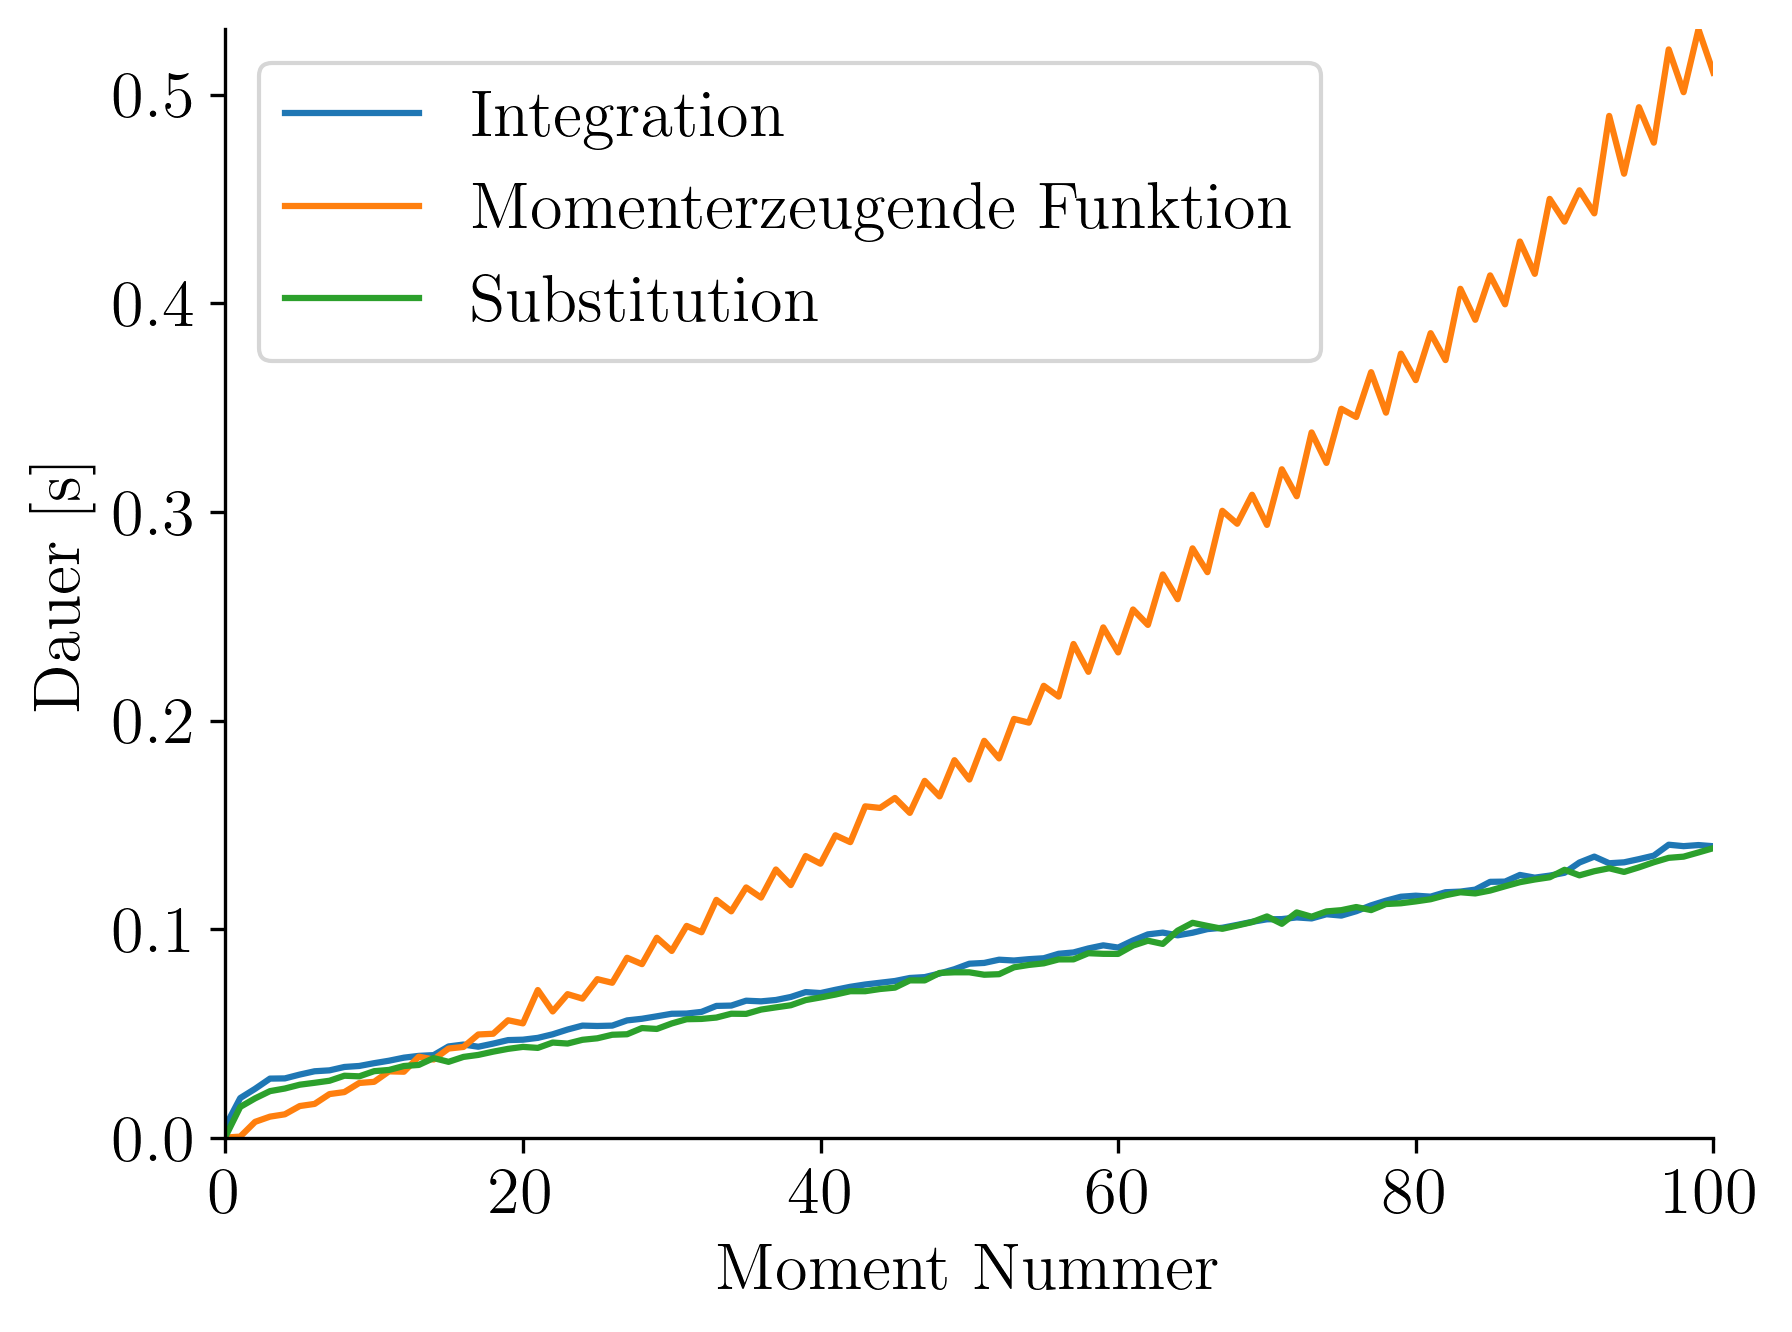
\includegraphics[width=0.5\linewidth]{./Section/Momente/Dauer Gleich.png}
\vspace*{-.3\baselineskip}
\caption{Dauer der Berechnung der ersten hundert Momente einer Gleichverteilung auf $[a, b]$}
\end{figure}

Wir erkennen nun etwas scheinbar Überraschendes. Die Berechnung mittels der momenterzeugenden Funktion ist langsamer. Die Berechnung mittels Integration und Substitution scheinen wieder lineares Wachstum zu haben und sind interessanterweise gleich schnell. Die Berechnung mit der momenterzeugenden Funktion scheint quadratischen Aufwand zu haben.
\end{Beispiel}

Nun werden wir uns ein finites Beispiel anschauen.

\begin{Beispiel}{(Laufzeit Bernoulli-Verteilung)}
Sei $X \sim \Ber(p)$ mit $p \in (0, 1)$ Bernoulli-verteilt. Lassen wir die ersten hundert Momente tausendmal berechnen, so erhalten wir die folgende Grafik.

\begin{figure}[H]
\centering
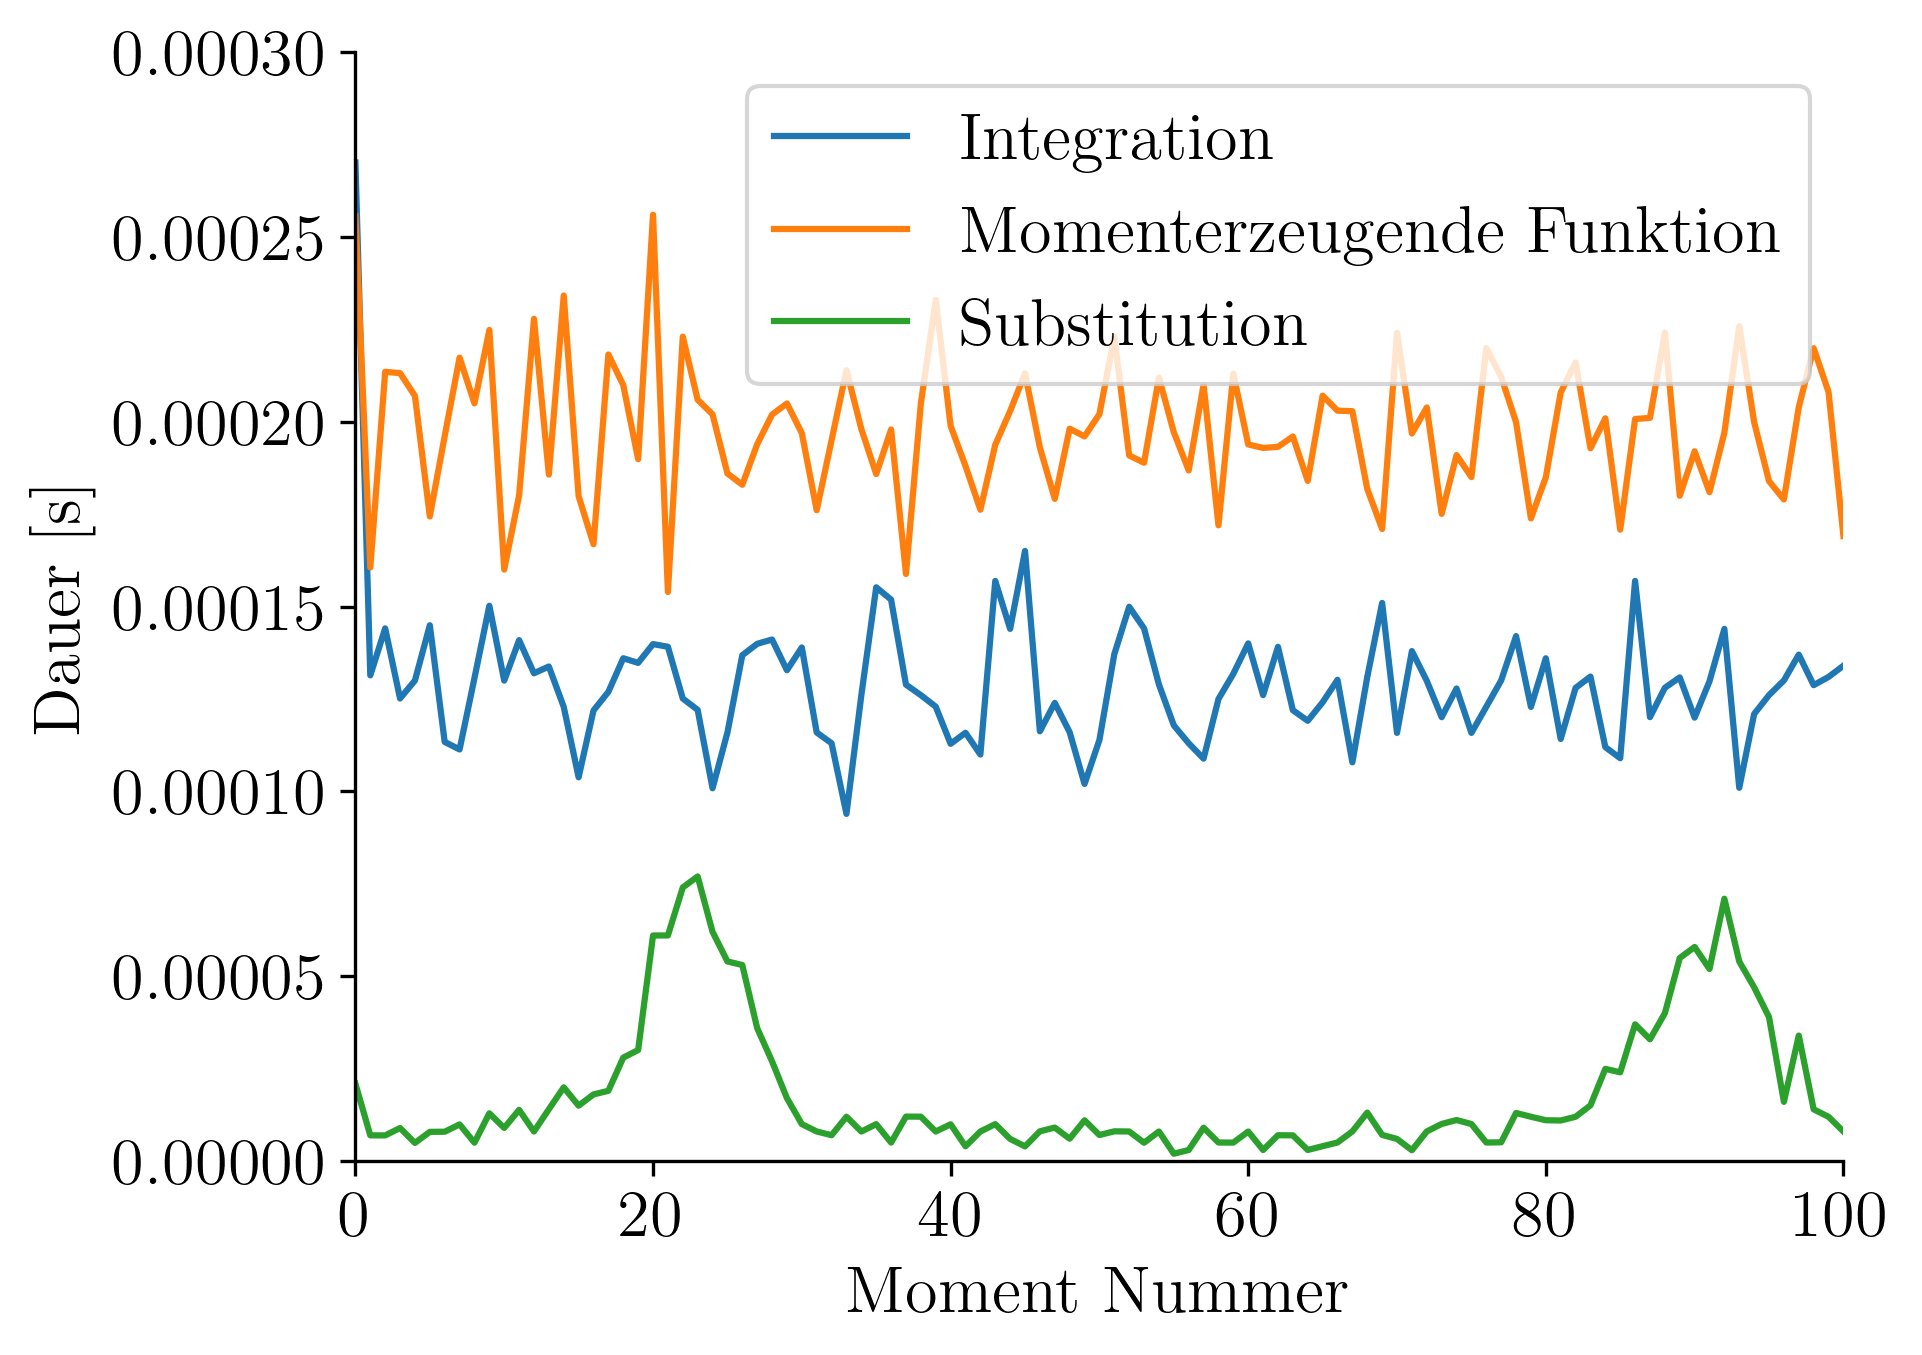
\includegraphics[width=0.5\linewidth]{./Section/Momente/Dauer Ber.png}
\vspace*{-.3\baselineskip}
\caption{Dauer der Berechnung der ersten hundert Momente einer $\Ber(p)$-Verteilung}
\end{figure}

Dieses Beispiel ist eher zum Spaß gedacht. Wir sehen, dass die Dauer der Berechnung im Zehntel Millisekundenbereich liegt. Diese unglaubliche Geschwindigkeit lässt sich darauf zurückführen, dass hier nur simpelste Berechnungen durchgeführt werden müssen. Es muss null oder eins potenziert werden und anschließend mit $1 - p$ respektive $p$ multipliziert werden. Aufgrund dieser Geschwindigkeit sind die Daten auch so rauschend, da die gesamte Berechnung nur wenige Sekunden gedauert hat und somit kleinste Nebentätigkeiten des Betriebssystem große Schwankungen hervorrufen. Vermutlich ist die Berechnung der Momente aller finiten Verteilungen derart \glqq einfach\grqq{}, da hier wie gesagt nur die Grundoperationen benötigt werden und diese sehr gut optimiert sind.
\end{Beispiel}

Als letztes Beispiel werden wir eine diskrete Zufallsvariable betrachten.

\begin{Beispiel}{(Laufzeit Poisson-Verteilung)}
Sei $X \sim \Poiss(\lambda)$ mit $\lambda > 0$ Poisson-verteilt. Hier lassen wir nur die ersten zwanzig Moment zehnmal berechnen. Wir erhalten den folgenden Plot.

\begin{figure}[H]
\centering
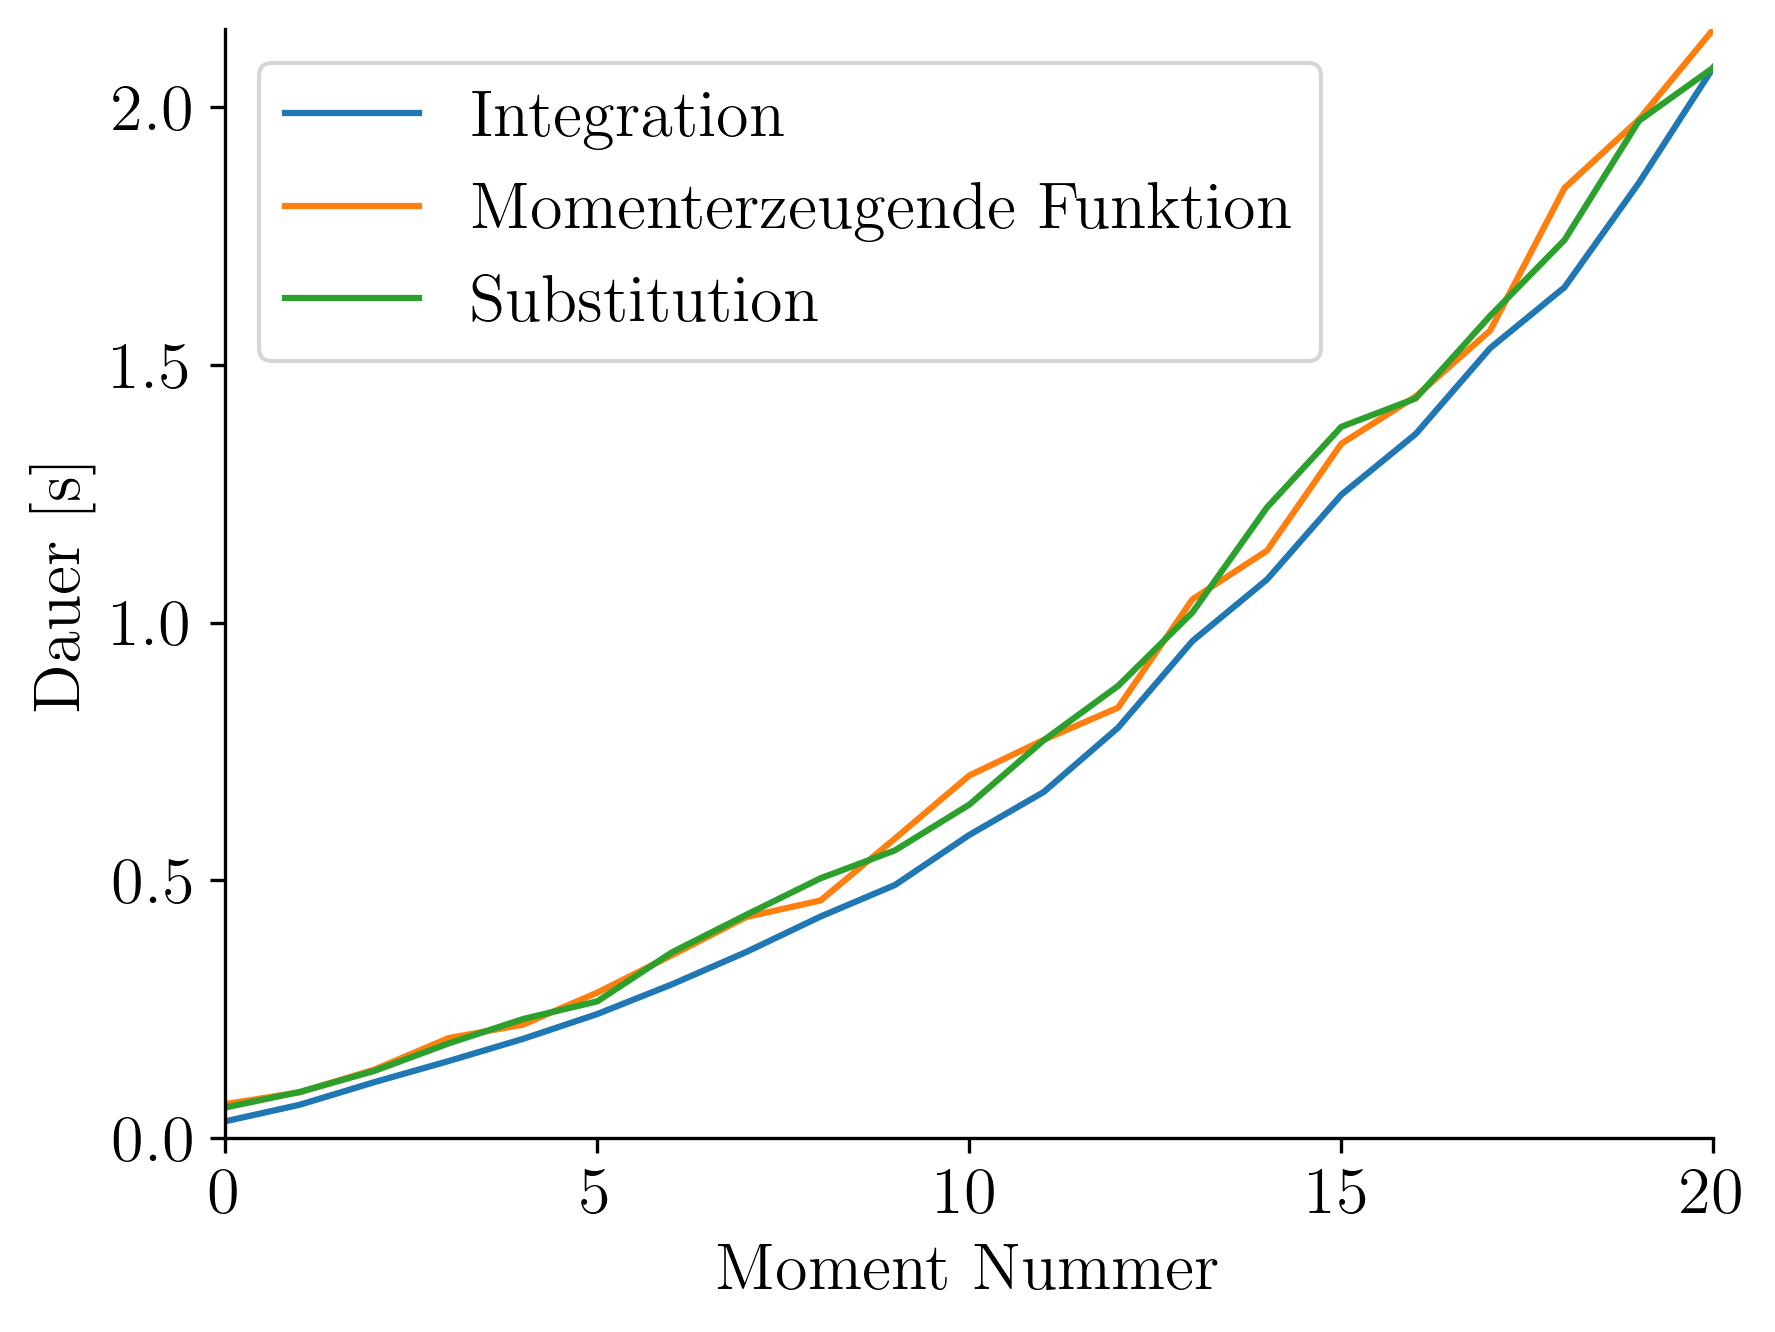
\includegraphics[width=0.5\linewidth]{./Section/Momente/Dauer Poisson.png}
\vspace*{-.3\baselineskip}
\caption{Dauer der Berechnung der ersten zwanzig Momente einer $\Poiss(\lambda)$-Verteilung}
\end{figure}

Interessanterweise sind hier alle drei Arten der Berechnung ziemlich genau gleich schnell und zeigen mindestens quadratisches Wachstum. Vermutlich sind alle Berechnungen ungefähr gleich schnell, da SymPy für Summen beziehungsweise Reihen keine so starken Werkzeuge hat, wie für Integrale. Dies ist vermutlich auch der Grund, wieso schon das zwanzigste Moment über $2$ Sekunden Rechenzeit benötigt.
\end{Beispiel}

Man stellt sich jetzt natürlich die Frage, was wir aus all diesen Beispielen gelernt haben. Es ist leider nicht klar, welche der Methoden \glqq die Beste\grqq{} ist. Je nach Verteilung ist eine andere Methode am schnellsten. Außerdem haben wir gelernt, dass finite Verteilungen blitzschnell berechenbar sind und diskrete Verteilungen scheinbar größere Probleme machen, wobei dies noch etwas näher beleuchtet werden sollte. Bei stetigen Verteilungen ist von der Rechendauer alles dabei.
